% We switch to portrait mode. This works as advertised.
\documentclass[a0,portrait]{a0poster}
% You might find the 'draft' option to a0 poster useful if you have
% lots of graphics, because they can take some time to process and
% display. (\documentclass[a0,draft]{a0poster})

\usepackage[utf8]{inputenc}

% Switch off page numbers on a poster, obviously, and section numbers too.
\pagestyle{empty}
\setcounter{secnumdepth}{0}

%fonts
\usepackage[T1]{fontenc}
\usepackage[oldstylenums, largesmallcaps]{kpfonts}
\renewcommand*\sfdefault{ugq}



%proper math and math symbols
%\usepackage{amsmath}
\usepackage{amssymb}

\usepackage{siunitx}

\usepackage{multirow}

% Allow the usage of graphics (.jpg, .png, etc.) in the document
\usepackage{graphicx}
\usepackage{tikz}
\usetikzlibrary{arrows,shapes,backgrounds, positioning, intersections, decorations.markings, decorations.shapes, mindmap, shapes.geometric, matrix, patterns}

\usepackage{pgfplots}
%\usepgfplotslibrary{units}
\usepgfplotslibrary{groupplots}
\pgfplotsset{every axis/.append style={xlabel near ticks,ylabel near ticks}}
\definecolor{BlueViolet}{rgb}{0.62352, 0.372549, 0.623529}

\definecolor{Maroon}{cmyk}{0, 0.87, 0.68, 0.32}
\usepackage{ragged2e}
\RaggedRight
% see documentation for a0poster class for the size options here
\let\Textsize\normalsize
\def\Head#1{\noindent\hbox to \hsize{\hfil{\LARGE\color{Maroon}\raggedright\textothersc{#1}}}\bigskip}
\def\LHead#1{\noindent{\LARGE #1}\smallskip}
\def\Subhead#1{\noindent{\large\textsf{#1}}}
\def\Title#1{\noindent{\VeryHuge\color{Maroon}\raggedright\textothersc{#1}}}

% The textpos package is necessary to position textblocks at arbitary 
% places on the page.
\usepackage[absolute,overlay,showboxes
]{textpos}
% Set up the grid
%
% Note that [40mm,40mm] is the margin round the edge of the page --
% it is _not_ the grid size. That is always defined as 
% PAGE_WIDTH/HGRID and PAGE_HEIGHT/VGRID. In this case we use
% 15 x 25. This gives us a wide central column for text (7 grid
% spacings) and two narrow columns (3 each) at each side for 
% pictures, separated by 1 grid spacing.
%
% Note however that texblocks can be positioned fractionally as well,
% so really any convenient grid size can be used.
%
\TPGrid[40mm,40mm]{15}{25}  % 3 - 1 - 7 - 1 - 3 Columns

% Mess with these as you like
\parindent=0pt
%\parindent=1cm
\parskip=0.5\baselineskip

\usepackage{paralist}

%bibliography
\usepackage{natbib}
\usepackage{bibentry}
\def\newblock{\hskip .11em plus .33em minus .07em}


%\includeonly{}

\begin{document}
%\tikzset{every mark/.append style={scale=0.8}}
%\pgfplotsset{every axis/.append style={small}}

\bibliographystyle{notitle}
\nobibliography{sift}

% Understanding textblocks is the key to being able to do a poster in
% LaTeX. In
%
%    \begin{textblock}{wid}(x,y)
%    ...
%    \end{textblock}
%
% the first argument gives the block width in units of the grid
% cells specified above in \TPGrid; the second gives the (x,y)
% position on the grid, with the y axis pointing down.

% You will have to do a lot of previewing to get everything in the 
% right place.

% This gives good title positioning for a portrait poster.
% Watch out for hyphenation in titles - LaTeX will do it
% but it looks awful.
\begin{textblock}{15}(0,0)
%\baselineskip=3\baselineskip \Title{
%Effects\,\textit{\Huge of a}\,real world size distribution\\
%\textit{\Huge on the}\,heterogeneous crystallisation\\
%\textit{\Huge of}\,hard sphere colloids\\}
\baselineskip=3\baselineskip \Title{
\begin{tabular}{rl}
Effects\,\textit{\Huge of a} & real world size distribution\\
\textit{\Huge on the} & heterogeneous crystallisation\\
\textit{\Huge of} & hard sphere colloids
\end{tabular}
}
\end{textblock}

\begin{textblock}{11}(0,3)
\LHead{
\begin{tabular}{lp{1.2em}l}
Mathieu Leocmach && \textothersc{Laboratoire de Physique -- UMR 5672,}\\
&& \textothersc{Ecole Normale Supérieure de Lyon}\hfill\texttt{\normalsize mathieu.leocmach@ens-lyon.fr}\\
Hajime Tanaka && \textothersc{Institute of Industrial science, The University of Tokyo}
\end{tabular}
}
\end{textblock}

\begin{textblock}{2.5}(12.5,0.65)
\begin{center}

\includegraphics[width=0.5\columnwidth]{QRcode}
\end{center}
\textit{Soft Matter}, 9, 1447--1457 (2013)
\end{textblock}


%Our colloids
\begin{textblock}{3}(4,4.5)
	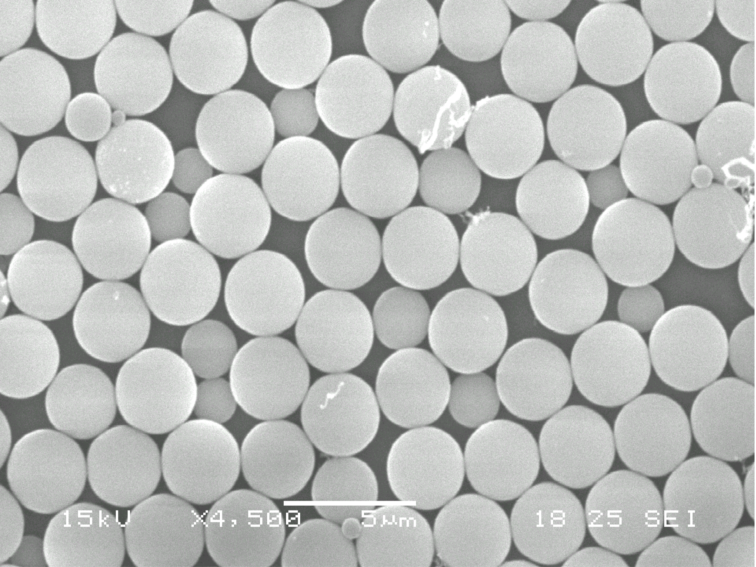
\includegraphics[width=\columnwidth]{SEM.pdf}
	
	\centering
	S.E.M. image
\end{textblock}
\begin{textblock}{3}(0,4.5)
	\Head{Our colloids}
	Index \& density-matched solvent
	\begin{itemize}
		\item Cis-decalin
		\item Cyclohexylbromide
	\end{itemize}
	PMMA particles $\approx$ Hard spheres
	\begin{itemize}
		\item Sterically stabilized
		\item Salt to screen charges\\ (Debye length $<\SI{100}{\nano\metre}$)
	\end{itemize}
\end{textblock}

\begin{textblock}{3}(8,4.5)
	\Head{Size distribution}
	%\tikzset{external/force remake=false}
	\begin{tikzpicture}
	\begin{axis}[%
		name=hist,
		width=\columnwidth, height=0.7\columnwidth,%
		%scale only axis,
		xlabel={Diameters [$\si{\micro\metre}$]},%
		xmin=1, xmax=5,
		axis y line*=left,
		ymin=0, ytick=\empty,%
		ylabel={Size distribution},%
		ylabel near ticks,
		legend style={legend pos=north west}, area legend,
		]
		\addplot[ybar, ybar interval, gray!50, fill=gray!50] file {SEM_size_distrib.txt} \closedcycle;
		\legend{\textsc{sem}}
	\end{axis}
	\begin{axis}[%
		name=hist2,
		width=\columnwidth, height=0.7\columnwidth,%
		xmin=1, xmax=5,
		axis y line*=right,
		ymin=0, ytick=\empty,%
		no marks,%
		]
		\addplot+[dashed] table[x expr ={2*\thisrow{r}}, y=all] {all_ico_icongb_mrco_X.rdist};
		\addlegendentry{In situ};
		\addplot table [x expr ={2*\thisrow{r}/1.25}, y index=1] {all_ico_icongb_mrco_X.rdist};
		\draw[->, ultra thick] (axis cs:3.15,3) -- (axis cs: 3.9, 3) node[midway, above] {swelling};%
	\end{axis}
	\end{tikzpicture}
\end{textblock}

\begin{textblock}{3}(0,8)
	\Head{Buoyancy control}
	\Subhead{by temperature control}
	\begin{itemize}
	\item Find $T_\text{matching}$ (a few days)
	\item $T>T_\text{matching}$
	\begin{itemize}
		\item makes particles sink
		\item melts the crystals at the top
	\end{itemize}
	\item Back to $T_\text{matching}$
	\end{itemize}
	$\Rightarrow$ observe crystallisation from the \linebreak beginning.
\end{textblock}

\begin{textblock}{3}(0,11.5)
	\Head{Local structures}
	Identified using bond orientational order
	
	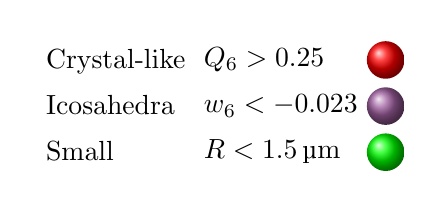
\begin{tikzpicture}
		\matrix[%
		matrix of nodes, ampersand replacement=\&,
		column 1/.style={right, text height=0.8em, text depth=0.2em},%
		column 2/.style={right},
		column 3/.style={left, circle, shade, inner sep=0.4\baselineskip},%
		] (l)
	{
		Crystal-like \& $Q_6>0.25$ \& |[ball color=red]|{}\\
		Icosahedra \& $w_6<-0.023$ \& |[ball color=BlueViolet]|{}\\
		Small \& $R<\SI{1.5}{\micro\metre}$ \& |[ball color=green]|{}\\
	};
	\end{tikzpicture}
\end{textblock}

\begin{textblock}{7}(4,8)
	\Head{Structure visualisation}
	\begin{tikzpicture}
		\node[anchor=south east, inner sep=0] at (-0.5\TPHorizModule,0) (t000) {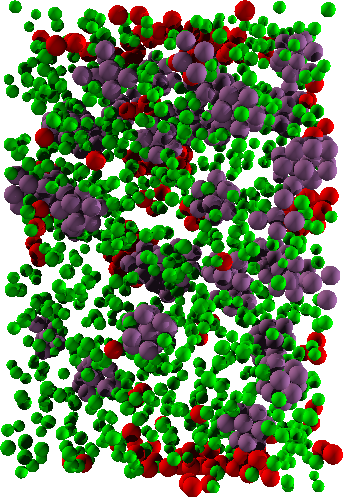
\includegraphics[width=3\TPHorizModule]{mrco_ico_small_t000.png}};
		\node[anchor=south west, inner sep=0] at (0.5\TPHorizModule,0) (t299) {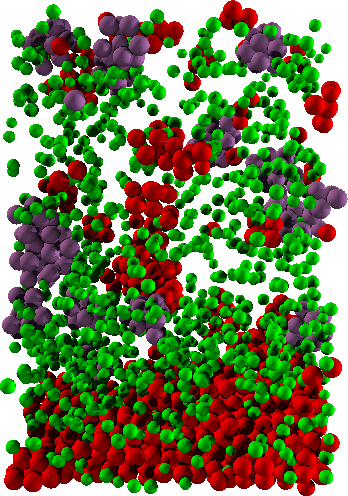
\includegraphics[width=3\TPHorizModule]{mrco_ico_small_t299.png}};
		\node[below=0 of t000.south] {$t=0$};
		\node[below=0 of t299.south] {$t=\SI{40}{\hour}$};
		\draw[->, very thick] (0,\TPVertModule) -- (0,3\TPVertModule) node[above]{$z$};
	\end{tikzpicture}
\end{textblock}

\begin{textblock}{3}(12,8)
	\Head{Size distributions}
	\Subhead{within local structures}
	
	\begin{tikzpicture}[
		%lab/.style={above right, text height=0.8em, text depth=0.2em, font=\Large\bfseries}%
		]%
	\begin{groupplot}[%
		group style={
			group name=distrib,
			group size=1 by 2,
			vertical sep=0.9\TPVertModule,
			},%
		width=\columnwidth,%
		height=0.6\columnwidth,%
		no marks,%
		xlabel={$R$ [$\si{\micro\metre}$]}, xmin=0.8, xmax=2.5,%
		ylabel={Size distribution}, ymin=0, ymax=12, ytick=\empty,%
		legend style={legend pos=north west},
		]
		\nextgroupplot
		\addplot[gray!50,fill=gray!50, area legend] table[x=r, y=all] {all_ico_icongb_mrco_X.rdist} \closedcycle;
		\addplot[dashed,red] table[x=r, y=mrco] {all_ico_icongb_mrco_X.rdist};
		\addplot[brown, very thick] table[x=r, y=X] {all_ico_icongb_mrco_X.rdist};
		\legend{all, crystal-like, crystalline};
		
		\nextgroupplot
		\addplot[gray!50,fill=gray!50, area legend] table[x=r, y=all] {all_ico_icongb_mrco_X.rdist} \closedcycle;
		\addplot[dashed,blue] table[x=r, y=ico] {all_ico_icongb_mrco_X.rdist};
		\addplot[BlueViolet, very thick] table[x=r, y=icongb] {all_ico_icongb_mrco_X.rdist};
		\legend{all, ico. centre, ico. surf.};
	\end{groupplot}
	%\node[lab, above right=0 of distrib c1r1.outer south west] {a};
	%\node[lab, above right=0 of distrib c1r2.outer south west] {b};
	\end{tikzpicture}
\end{textblock}

\textblockcolour{lightgray!50!white}
\TPMargin*{ 0.125\TPHorizModule }
\begin{textblock}{2.875}(12,3.125)%real width of 3
	\Head{Conclusion}
	\Subhead{A relyable method to}
	\begin{itemize}
		\item track particles even when
		\begin{itemize}
			\item arbitrary size distribution
			\item high density
		\end{itemize}
		\item measure the sizes
		\begin{itemize}
			\item of each particles
			\item in situ
		\end{itemize}
	\end{itemize}
	\Subhead{Small particles}
	\begin{itemize}
		\item promote icosahedral order for a size ratio of 0.8
		\item must be expelled before crystal-like ordering
		\item induce polycrystalline material
	\end{itemize}
	
	%\textsf{The crystal is important} to understand the glass.
\end{textblock}%Conclusion

%Central block of 3D reconstructions
%\begin{textblock}{7}(4,7)
%	\Head{Reconstruction from experimental coordinates}
%	Colloidal hard spheres (\textsc{pmma} in cis-decalin and \textsc{chb} with \textsc{tbab}) are tracked by confocal microscopy. Diameter is $\approx\SI{3}{\micro\metre}$ and polydispersity is $\approx 6\%$ to avoid crystallisation.
%	
%	\begin{tikzpicture}[%
%		pic3d/.style={inner sep=0}, %
%		lab/.style={below left=0.002\textwidth and 0.005\textwidth, text height=0.8em, text depth=0.2em, font=\bfseries},%
%		arr/.style={<->, thick, yellow!75!black}%
%		]%
%	\definecolor{turquoise}{rgb}{0.678431,0.917647,0.917647}
%	\node[below left, pic3d] at(0.5\textwidth,0.5\textwidth) (all) {\includegraphics[width=0.48\textwidth]{mrco_ico_scale_go1-0023.png}};
%	\node[above left, pic3d] at (0.5\textwidth,-0.5\textwidth) (dyn) {\includegraphics[width=0.48\textwidth]{cgsd_2tau.png}};
%	\node[above right, pic3d] at (-0.5\textwidth,-0.5\textwidth) (mrco) {\includegraphics[width=0.48\textwidth]{mrco24_scale_go1_t040_t048.png}};
%	\draw [help lines, step=0.12\textwidth, shift=(mrco.south west)] (0, 0) grid (0.48\textwidth, 0.48\textwidth);
%	\draw [help lines, step=0.12\textwidth, shift=(dyn.south west)] (0, 0) grid (0.48\textwidth, 0.48\textwidth);
%	\node[below left=0.5em of dyn.south east] {$10\%$ slowest particles};
%	\node[below right=0.5em of mrco.south west] {$10\%$ most crystal-like};
%	\node[below] at (0,-0.5\textwidth){\textsf{Spatial correlation}};
%	\matrix[%
%		matrix anchor=east, draw,% 
%		column 1/.style={text height=0.8em, text depth=0.2em},%
%		column 2/.style={circle, shade, inner sep=0.008\textwidth},%
%		] at (-0.02\textwidth, 0.25\textwidth) (l)
%	{
%		\node{Icosahedra}; & \node[ball color=red!50!blue] (b2) {};\node[ball color=red!75!black, left] at (b2.west) {}; \node[ball color=blue!75!black, right] at (b2.east) {};\\
%		\node{Crystal-like}; & \node[ball color=green!66!black] {}; \\
%		\node{Slow}; & \node[ball color=turquoise!75!black] {}; \\
%	};
%	\node[below right, pic3d] at (-0.5\textwidth,0.5\textwidth) (one_ico) {\includegraphics[width=0.22\textwidth]{one_ico.png}};
%	\node[below left, text width=0.2\textwidth, align=right, inner sep=0] at(-0.02\textwidth, 0.5\textwidth) {Icosahedral\\ order is \textsf{local}};
%	\node[right=0.01\textwidth] at (one_ico.east){$w_6=w_6^*$};
%	\node[above right, pic3d] at (-0.5\textwidth,0) (one_mrco) {\includegraphics[width=0.22\textwidth]{one_mrco.png}};
%	\node[above left, text width=0.2\textwidth, align=right, inner sep=0] at(-0.02\textwidth,0.02\textwidth) {Crystal-like clusters reach \textsf{medium range}};
%	\node[right=0.01\textwidth] at (one_mrco.east) {$Q_6=Q_6^*$};
%	\end{tikzpicture}
%\end{textblock}
%
%%Glass transition, cooling curve
%%\begin{textblock}{3}(0,3.5)
%%	\begin{tikzpicture}[
%%		temp/.style={circle, inner sep=0.01\columnwidth, outer sep=0, fill=magenta},%
%%		label position=below right, label distance=-0.03\columnwidth,%
%%		]
%%	\begin{axis}[%
%%		width=\columnwidth, height=0.8\columnwidth,%
%%		xlabel=Temperature, xmin=0, xmax=1.2, axis x line=bottom, xtick=\empty,%
%%		extra x ticks={0.2, 0.45, 0.7, 0.95}, extra x tick labels={$T_0$, $T_g$,,$T_m$}, xlabel near ticks,%
%%		ylabel=Entropy, ymin=0.1, ymax=1.2, axis y line=left, ytick=\empty, ylabel near ticks,%
%%		]
%%		\draw (axis cs:0, 0.18) -- (axis cs:0.95, 0.28);
%%		\draw (axis cs:0.45, 0.45) -- (axis cs:1.2,1.2);
%%		\draw[dotted] (axis cs:0.2, 0.2)-- (axis cs:0.45, 0.45);
%%		\draw[help lines] (axis cs:0.2, 0)-- (axis cs:0.2, 0.2);
%%		\draw[help lines] (axis cs:0.45, 0)-- (axis cs:0.45, 0.45);
%%		\draw[help lines] (axis cs:0.7, 0)-- (axis cs:0.7, 0.7);
%%		\draw[help lines] (axis cs:0.95, 0)-- (axis cs:0.95, 0.95);
%%		\draw[red] (axis cs:0.45, 0.45) to [out=225, out looseness=0.2, in=5] (axis cs:0,0.35);
%%		\draw[orange] (axis cs:0.45, 0.45) to [out=225, out looseness=0.5, in=5] (axis cs:0,0.325);
%%		\draw[yellow] (axis cs:0.45, 0.45) to [out=225, out looseness=0.8, in=5] (axis cs:0,0.3);
%%		\node[temp, label=\tiny{$\tau\sim10^{-13}$}] at (axis cs:0.95, 0.95) {};
%%		\node[temp, label=\tiny{$\tau\sim10^{-9}$}] at (axis cs:0.7, 0.7) {};
%%		\node[temp, label=\tiny{$\tau\sim10^{3}$}] at (axis cs:0.45, 0.45) {};
%%		\node[temp, label=\tiny{$\tau\rightarrow\infty$?}] at (axis cs:0.2, 0.2) {};
%%		\node[above, anchor=south] at (axis cs:0.15, 0.34) (gl) {\small{glass}};
%%		\node[above, anchor=south, rotate=41.5] at (axis cs:0.7,0.7) {\small{supercooled liquid}};
%%		\node[above, anchor=south west, rotate=41.5] at (axis cs:0.95,0.95) {\small{liquid}};
%%		\node[below, anchor=north east] at (axis cs:0.95,0.28) {\small{crystal}};
%%	\end{axis}
%%	\end{tikzpicture}
%%\end{textblock}
%\begin{textblock}{3}(0,3)
%	\Head{Motivation}
%	\Subhead{Structural cause}
%	\begin{itemize}
%		\item dynamic heterogeneity
%		\item dynamic length scale
%		\item dynamical arrest
%	\end{itemize}
%	
%	For each structure candidate, \\a different theory
%	\begin{itemize}
%		\item order from the liquid
%		\item order from the crystal
%		\item exotic%\\{\footnotesize\bibentry{lubchenko2007}}
%	\end{itemize}
%\end{textblock}
%
%\begin{textblock}{5}(4,3)
%	\Head{Liquid's locally favoured structures}
%\end{textblock}
%\begin{textblock}{1.5}(4,3.5)
%	Cannot fill space because of geometrical frustrations
%
%\begin{center}\begin{tikzpicture}[pen/.style={regular polygon, regular polygon sides=5, draw, minimum size=4em}]
%	\node[pen] (base) {};
%	\node[pen,anchor=south, rotate=180] at (base.side 3) {};
%	\node[pen,anchor=south, rotate=-108] at (base.side 4) {};
%\end{tikzpicture}\end{center}
%	Domain size\\
%	Defect size
%\end{textblock}
%\begin{textblock}{3}(6,3.5)
%	Theories
%	\begin{itemize}
%	\raggedright
%	\item Spin-glass type\\{\footnotesize\bibentry{steinhardt1983boo}}
%	\item Frustration-limited domain\\{\footnotesize\bibentry{tarjus2005fba}}
%	\end{itemize}
%	Canonical example: \textsf{Icosahedron}
%	
%	\begin{center}
%	\includegraphics[height=\TPVertModule]{d20}
%	\end{center}
%\end{textblock}
%
%
%\begin{textblock}{1.5}(9.5,3)
%\Head{Tracking}
%\begin{center}
%\includegraphics[height=2\TPVertModule]{comp2D3D_crop2}
%\end{center}
%
%Tracking precision in \textsf{position and size} is $\approx \sigma/100$.
%%\includegraphics[height=\textwidth]{Dzugutov_LFS}\\
%%{\footnotesize \bibentry{Dzugutov2002}}
%\end{textblock}
%
%\begin{textblock}{3}(0,7)
%	\Head{Crystal-like order}
%	\begin{tikzpicture}[inner sep=0]
%	\node[left, text width=0.7\textwidth] at(10.5,-7){
%	Cannot fill space because
%	\begin{itemize}
%		\item Energy barrier
%		\item Other structures locally more stable
%		\item Kinetic barrier
%		\item Size polydispersity
%	\end{itemize}};
%	\begin{scope}[scale=0.25, rotate=-90]
%			\tikzset{particle/.style={circle, ball color=blue!50!white, inner sep=0, minimum size=1em}}
%			\tikzset{ar/.style={->, draw=red!80!black, ultra thick}}
%			\node[particle] at (14.356, 47.436) (a) {};
%			\node[particle] at (17.000, 52.387) (b) {};
%			\node[particle] at (20.000, 48.000) (c) {};
%			\node[particle] at (17.178, 44.149) (d) {};
%			\node[particle] at (22.258, 51.951) (e) {};
%			\node[particle] at (22.822, 44.049) (f) {};
%			\node[particle] at (23.387, 56.467) (g) {};
%			\node[particle] at (27.902, 58.160) (g1) {};
%			\node[particle] at (26.773, 53.080) (h) {};
%			\node[particle] at (25.644, 48.000) (i) {};
%			\node[particle] at (31.300, 54.773) (j) {};
%			\node[particle] at (30.724, 49.693) (k) {};
%			\node[particle] at (36.000, 57.596) (k1) {};
%			\node[particle] at (35.804, 53.016) (l) {};
%			\node[particle] at (34.676, 47.436) (m) {};
%			\node[particle] at (40.320, 54.209) (n) {};
%			\node[particle] at (39.191, 49.129) (o) {};
%			\path[ar] (d) edge (c);
%			\path[ar] (c) edge (e);
%			\path[ar] (i) edge (h);
%			\path[ar] (k) edge (j);
%			\path[ar] (l) edge (k1);
%			\draw[green!50!black, ultra thick] (a) -- (c) -- (b);
%			\path[green!50!black,<->, ultra thick] (a) edge [bend left] (b);
%			\draw[green!50!black, ultra thick] (n) -- (l) -- (o);
%			\path[green!50!black,<->, ultra thick] (n) edge [bend left] (o);
%	\end{scope}
%	\end{tikzpicture}%
%	
%	{\footnotesize\bibentry{tanaka2010critical}}\\
%	\begin{tikzpicture}
%	\fill[left color=yellow!30!black, right color=yellow] (-0.45\textwidth,0) rectangle (-0.1\textwidth,-0.5em);
%	\path (-0.45\textwidth,-0.5em) -- (-0.1\textwidth,-0.5em) 
%		node[below, pos=0] {\scriptsize $0.5$}
%		node[below, pos=0.33] {\scriptsize $0.6$}
%		node[below, pos=0.67] {\scriptsize $0.7$}
%		node[below, pos=1] {\scriptsize $0.8$};
%	\fill[left color=yellow!30!black, right color=yellow] (0.1\textwidth,0) rectangle (0.45\textwidth,-0.5em);
%	\path (0.1\textwidth,-0.5em) -- (0.45\textwidth,-0.5em) 
%		node[below, pos=0] {\scriptsize $0.6$}
%		node[below, pos=0.5] {\scriptsize $1.1$}
%		node[below, pos=1] {\scriptsize $1.6$};
%	\node[above right, inner sep=0] at(-0.5\textwidth,0.25em) (psi6) {\includegraphics[width=0.45\textwidth, height=0.45\textwidth]{kawa_nm_psi6.png}};
%	\node[above left, inner sep=0] at(0.5\textwidth,0.25em) (msd) {\includegraphics[width=0.45\textwidth, height=0.45\textwidth]{kawa_nm_msd.png}};
%	\node[below=1.5em of psi6] {$\Psi_6$};
%	\node[below=1.5em of msd] {$\Delta r^2$};
%	\end{tikzpicture}
%	
%	
%	\textothersc{\Large `Crystal' }is the symmetry breaking phase, avoided \emph{by definition} to get the supercooled liquid.
%	\begin{compactitem}\item Classical crystal (\textsc{fcc, hcp, bcc}\ldots)
%	
%	\begin{tikzpicture}[inner sep=0]
%	\node[text width=0.5\textwidth, right] at(0,0) (Qt) {\item Quasi-crystal};
%	\node[text width=0.5\textwidth, left] at(\textwidth,0) (FK) {\item Frank-Kasper};
%	\node[below=0em of Qt] (Quasi) {\includegraphics[height=0.25\textwidth]{Ho-Mg-ZnQuasicrystal.jpg}};
%	\node[below=0em of FK] (FrankKasper) {\includegraphics[height=0.25\textwidth]{frankkasper.png}};
%	\node[text width=0.4\textwidth, below=of Quasi] {for Dzugutov system\\{\footnotesize\bibentry{Doye2003}}};
%	\node[text width=0.4\textwidth, below=of FrankKasper] {for Wangstr\"om mixture\\{\footnotesize\bibentry{Pedersen2010}\\ \bibentry{Coslovich2011}}};
%	\end{tikzpicture}
%	
%	\item[$\Rightarrow$] `Crystal' may contain icosahedral motif\\
%	\item[$\Rightarrow$] Slow icosahedral clusters are \\crystal-like in these systems
%	\end{compactitem}
%
%\end{textblock}%Crystal-like order
%
%\begin{textblock}{4}(0,17)
%	\Head{In our hard spheres}
%	We have both a crystal (\textsc{fcc}) and icosahedral order. Orderings are orthogonal, incompatible and frustrate mutually.
%	
%	\begin{tikzpicture}
%		\pgfplotsset{
%			extra tick style={grid=major},%
%			every axis/.append style={%
%				height=0.5\textwidth,
%				ymin=0,ymax=0.6,%
%				extra y ticks={\Qstar}, extra y tick labels={},%
%				enlargelimits=false,axis on top,
%				colormap={bw}{gray(0cm)=(1); gray(1cm)=(1); gray(10cm)=(0)},%
%				colorbar sampled,%
%				},%
%		}
%		\begin{groupplot}[
%			group style={
%				group name=gp,%
%				group size=2 by 1,%
%				yticklabels at=edge left,%
%				horizontal sep=0pt,%
%				},%
%			anchor=above north west,%
%			width=0.43\textwidth,%
%			xlabel={},%
%			xmin=-0.052,xmax=0.01,%
%			xtick={-0.05,-0.03,-0.01},%
%			extra x ticks={\wstar, -0.00782},%
%			extra x tick labels={,},%
%			xtick scale label code/.code={},%
%			colorbar right, colorbar style={%
%				samples=6, ytick={ 0.20,0.4,0.6, 0.8},% 
%				yticklabels={$10^{1}$, $10^{2}$, $10^{3}$, $10^{4}$},%
%				%ylabel={per units of $w_6\cdot Q_6$},%
%				extra x ticks={},%
%				extra y ticks={},%
%				label style={font=\footnotesize},
%				},%
%			]
%		\nextgroupplot[ylabel={Crystal-like ($Q_6$)}, ylabel near ticks]
%		\addplot graphics
%		[xmin=-0.052,xmax=0.052,ymin=0,ymax=0.6]
%		{u6Q6phi3954_scale};
%		\node [above] at (axis cs:-0.04, \Qstar) {\footnotesize{$Q_6^*$}};
%		%\node [anchor=north east] at (rel axis cs:1, 1) {\footnotesize{$\phi = 0.497 \pm 0.03$}};
%		\node [left] at (axis cs:\wstar,0.4) {\footnotesize $w_6^*$};
%		\node [right] at (axis cs:-0.00782,0.4) {\footnotesize $w_6^{dod}$};
%		
%		\nextgroupplot
%		\addplot graphics
%		[xmin=-0.052,xmax=0.052,ymin=0,ymax=0.6]
%		{u6Q6go1_scale};
%		\node at (axis cs:\wstar,0.6) (a) {};
%		\node at (axis cs:-0.00782,0.6) (b) {};
%		\node [below] at (axis cs:-0.0026, 0.5745) {\textsc{fcc}};
%		\node [below, right] at (axis cs:-0.052, 0.05) {\textsc{Ico}};
%		\draw[->, green,line width=0.15em, semitransparent] (axis cs:-0.001, 0.15) to [out=90, in=275] (axis cs:-0.0015, 0.33);
%		\draw[->, purple,line width=0.15em, semitransparent] (axis cs:-0.001, 0.15) to [out=180, in=30] (axis cs:-0.025, 0.12);
%		\end{groupplot}
%		\node[below=of gp c1r1.south east]{Icosahedral ($10^2 \cdot w_6$)};
%		\node[above=0 of gp c1r1.north] {Normal liquid};
%		\node[above=0 of gp c2r1.north] {Deep supercooling};
%		\end{tikzpicture}
%		\begin{tikzpicture}
%		\pgfplotsset{
%			extra tick style={grid=major},%
%			every axis/.append style={%
%				height=0.48\textwidth,
%				ymin=0,ymax=0.6,%
%				extra y ticks={\Qstar}, extra y tick labels={},%
%				enlargelimits=false,axis on top,
%				colormap={bw}{gray(0cm)=(1); gray(1cm)=(1); gray(10cm)=(0)},%
%				colorbar sampled,%
%				},%
%			}
%		\begin{groupplot}[
%			group style={
%				group size=2 by 1,%
%				yticklabels at=edge left,%
%				horizontal sep=0pt,%
%				},%
%			width=0.48\textwidth,%
%			xtick scale label code/.code={},%
%			colorbar horizontal, colorbar style={%
%				samples=6, xtick={ 0.20,0.4,0.6, 0.8},% 
%				extra y ticks={},%
%				/pgfplots/colorbar shift/.style={yshift=0.3cm},
%				at={(parent axis.north)}, anchor=below south, width=0.9*\pgfkeysvalueof{/pgfplots/parent axis width},
%				xticklabel pos=upper,%
%				%label style={font=\footnotesize},
%				},%
%				xlabel near ticks,%
%			]
%		\nextgroupplot[%
%			ylabel={Crystal-like ($Q_6$)}, ylabel near ticks, xlabel=$Q_4$, %
%			xmin=0,xmax=0.22,%
%			colorbar style={%
%				xlabel={},% 
%				xticklabels={$10^{1}$, $10^{2}$, $10^{3}$, $10^{4}$},%
%				},%
%			xticklabel={$\pgfmathprintnumber[fixed,precision=2]{\tick}$}
%			]
%		\addplot graphics
%		[xmin=0,xmax=0.2,ymin=0,ymax=0.6]
%		{Q4Q6go1};
%		\node [below] at (axis cs:0.1909, 0.5745) {\textsc{fcc}};
%		\node [below] at (axis cs:0.0972222, 0.484762) {\textsc{hcp}};
%		\node [below] at (axis cs:0.0363696, 0.510688) {\textsc{bcc}};
%		\draw[->, green,line width=0.15em, semitransparent] (axis cs:0.05, 0.15) to [out=60, in=220] (axis cs:0.125, 0.4);
%		
%		\nextgroupplot[%
%			xlabel=$10^3 \cdot w_4$, %
%			xmin=-0.002,xmax=0.002,%
%			xtickmin=-0.0015,%
%			xtick={-0.001,0,0.001},%
%			extra x ticks=0, extra x tick labels={},
%			colorbar style={%
%				xlabel={},% 
%				xticklabels={$10^{3}$, $10^{4}$, $10^{5}$, $10^{6}$},%
%				},%
%			]
%		\addplot graphics
%		[xmin=-0.002,xmax=0.002,ymin=0,ymax=0.6]
%		{w4Q6go1};
%		\node [below] at (axis cs:-0.00067221, 0.5745) {\textsc{fcc}};
%		\node [below] at (axis cs:7.47E-05, 0.484762) {\textsc{hcp}};
%		%\node [below] at (axis cs:-0.01274716, 0.510688) {\textsc{bcc}};
%		\node [above] at (axis cs:0.0015, \Qstar) {\footnotesize{$Q_6^*$}};
%		\draw[->, green,line width=0.15em, semitransparent] (axis cs:0, 0.15) to [out=120, in=280] (axis cs:-0.0005, 0.4);
%		\draw[->, green,line width=0.15em, semitransparent] (axis cs:0, 0.15) to (axis cs:7E-05, 0.35);
%		
%		\end{groupplot}
%	\end{tikzpicture}
%	
%	No exotic order.
%\end{textblock}%In our hard spheres
%
%\begin{textblock}{3}(12,9)
%	\Head{Dynamics}
%	
%	\raggedleft\begin{tikzpicture}
%		\begin{axis}[%
%			name=isf,%
%			anchor=north west,%
%			width=0.88\textwidth, height=0.33\textwidth, %
%			xlabel=$t/\tau_B$, xmode=log,%
%			ylabel={Self ISF}, ymin=0,%
%			xlabel near ticks, ylabel near ticks,%
%			%legend columns=3, reverse legend, legend style={font=\tiny, at={(1,1.03)}, anchor=south east}, %
%			]
%			\draw[->, line width=0.5em, lightgray] (axis cs:2, 0.35) -- (axis cs:5000, 0.35) node[black, right] {$\phi$};
%			\addplot file {LS3954.isf};
%			\addplot file {LS4446.isf};
%			\addplot file {LS4582.isf};
%			\addplot file {LS5079.isf};
%			\addplot file {go1.isf};
%			%\addlegendimage{legend image code/.code={\node[right] {$\phi\;\pm$};}};
%			%\legend{$0.497$, $0.535$, $0.540$, $0.555$, $0.575$, $0.003$};
%			
%		\end{axis}
%		\tikzset{every mark/.append style={scale=2}}
%		\begin{axis}[%
%			name=tau,%
%			anchor=north west,%
%			at={(isf.below south west)},%
%			width=0.88\textwidth, %
%			height=0.6\textwidth, %
%			xlabel=$\phi$, xmin=0.49, xmax=0.58,%
%			xtick={0.5,0.52,...,0.6},%
%			extra x ticks={0.495,0.545},%
%			extra x tick labels={},%
%			extra tick style={grid=major},%
%			ylabel=$\tau_\alpha/\tau_B$, ymode=log, %
%			xlabel near ticks, ylabel near ticks,%
%			legend pos=north west,%
%			%cycle list={{black, mark=*},{black, mark=square}},%
%			]
%			%\addplot+[mark=none, forget plot, domain=0.49:0.58] {0.7874243*exp(0.32826088*x/(0.60063652-x))};
%			\addplot+[only marks] table[x index=0, y index=1]{xi_phi.dat};
%			\addplot+[mark=none, black, domain=0.49:0.58] {exp(0.28970401*x/(0.59841615-x))};
%			\addplot+[only marks, mark=square, red] table[x index=0, y index=4]{xi_phi.dat};
%			\legend{Relaxation time, V.F.T. fit $\Rightarrow\phi_0$, Dynamic hetero.};
%		\end{axis}
%		\definecolor{turquoise}{rgb}{0.678431,0.917647,0.917647}
%		\begin{axis}[%
%			name=lengths,%
%			at={(tau.below south west)},% 
%			anchor=north west, %
%			width=0.88\textwidth, %
%			height=0.7\textwidth, %
%			xlabel=$\phi$, xmin=0.49, xmax=0.58, xlabel near ticks,%
%			xtick={0.5,0.52,...,0.6},%
%			extra x ticks={0.495,0.545},%
%			extra x tick labels={},%
%			extra tick style={grid=major},%
%			ylabel={Correlation length ($\xi/\sigma$)}, ymin=0, ymax=4.5,%
%			xlabel near ticks, ylabel near ticks,%
%			%legend pos=north west,%
%			cycle list={{turquoise!50!black, mark=*},{green!50!black, mark=square*}},%
%			]
%			\addplot+[mark=none, forget plot, domain=0.49:0.58] {0.41158778*((0.59773962-x)/0.59773962)^(-2.0/3.0)};
%			\addplot+[only marks] table[x index=0, y index=2]{xi_phi.dat};
%			\addplot+[mark=none, forget plot, domain=0.49:0.58] {0.18878182*((0.59773962-x)/0.59773962)^(-2.0/3.0)};
%			\addplot+[only marks] table[x index=0, y index=3]{xi_phi.dat};
%			\draw[decorate, decoration={%
%				text along path, text={dynamical}, text color=turquoise!50!black%
%				}] (axis cs:0.53,2.2) to [out=20, in=-120] (axis cs:0.57,4);
%			\draw[decorate, decoration={%
%				text along path, text={crystal-like order}, text color=green!50!black%
%				}] %
%				(axis cs:0.52,0.25) to [out=0, in=-140] (axis cs:0.58,1.25);
%			\node[below right=0.1em, fill=white, text width=0.45\textwidth] at (rel axis cs:0,1) {Same power law $\xi(\phi) \propto \xi_0 \left( \frac{\phi_0 - \phi}{\phi} \right)^{-\frac{2}{3}} $};
%			%\legend{$\xi_u$ dynamical, $\xi_6$ structural};
%		\end{axis}
%	\end{tikzpicture}
%	
%	\raggedright The divergence of the dynamics is linked to the crystal-like order
%\end{textblock}%Dynamics
%
%\begin{textblock}{10}(5,17)
%	\Head{Dynamics function of the initial structure}
%	\begin{tikzpicture}
%	\node at (-0.8\TPHorizModule,0) (a){};
%		\begin{axis}[%
%			name=Qw,%
%			anchor=right of south east,%
%			at=(a),%
%			width=1.73\TPHorizModule,%
%			height=2\TPHorizModule,%
%			ylabel={Crystal-like ($Q_6$)},%
%			ymin=0,ymax=0.6,%
%			xlabel={Icosahedral ($10^2 \cdot w_6$)},%
%			xmin=-0.052,xmax=0.01, xtickmax={0},%
%			xtick scale label code/.code={},%
%			xtick={-0.05,-0.03,-0.01},%
%			enlargelimits=false,axis on top,
%			colormap={sd}{color(0cm)=(black) rgb(1cm)=(0.5, 0, 0) rgb(2cm)=(1, 0.5, 0) color(3cm)=(yellow) rgb(4cm)=(0.5, 0.75, 1) rgb(5cm)=(0.5, 0.75, 1)},%
%			extra x ticks={\wstar, -0.00782},%
%			extra x tick style={grid=major,	tick label style={anchor=south west}},%
%			extra x tick labels={,},%
%			extra x tick style={grid=major},
%			extra y ticks={\Qstar},
%			extra y tick style={grid=major},
%			extra y tick labels={},%
%			colorbar sampled, colorbar style={%
%				samples=5, ytick={ 0, 0.25, 0.5, 0.75},% 
%				yticklabels={$0$, $0.5$, $1$, $1.5$},%
%				ylabel={Displacement},%
%				extra x ticks={},%
%				yticklabel pos=right,%
%				},%
%			xlabel near ticks, ylabel near ticks,%
%			]
%			\addplot graphics [xmin=-0.052,xmax=0.052,ymin=0,ymax=0.6]{sd_u6Q6_go1_color};
%			\node [above] at (axis cs:-0.04, \Qstar) {\footnotesize{$Q_6^*$}};
%			%\node [anchor=west] at (rel axis cs:0, 0.8) {\footnotesize{$\phi = 0.575 \pm 0.03$}};
%			\node [left] at (axis cs:\wstar,0.55) {\footnotesize $w_6^*$};
%			\node [left] at (axis cs:-0.00782,0.55) {\footnotesize $w_6^{dod}$};
%			\node [below] at (axis cs:-0.0026, 0.5745) {\textsc{fcc}};
%			\node [below, right] at (axis cs:-0.052, 0.05) {\textsc{Ico}};
%		\end{axis}
%		\pgfplotsset{every axis plot/.append style={only marks}}
%		\begin{groupplot}[%
%			group style={
%				group name=Q_w,%
%				group size=2 by 1,%
%				yticklabels at=edge left,%
%				horizontal sep=0pt,%
%				},%
%			anchor=left of south west,%			
%			width=2.15\TPHorizModule,%
%			height=2\TPHorizModule,%
%			ymin=0, ymax=1.5,%
%			extra x tick style={grid=major,	tick label style={anchor=south west}},%
%			extra y ticks={1},%
%			extra y tick style={grid=major,	tick label style={anchor=south west}}, extra y tick labels={},%
%			%legend columns=5,%
%			legend style={
%				font=\footnotesize,
%				%at={(1,1)}, anchor=south,%
%				at={(1,1)}, anchor=north east
%				},%
%			xlabel near ticks, ylabel near ticks,%
%			]
%			\nextgroupplot[%
%				xlabel={Icosahedral ($10^2 \cdot w_6$)}, xmin=-0.0521089193, xmax=0.01,%
%				xtick={-0.05,-0.03,-0.01,0},%
%				xtick scale label code/.code={},%
%				ylabel={},
%				extra x ticks={\wstar, -0.00782}, extra x tick labels={$w_6^*$,$w_6^{dod}$},%
%				extra y tick labels={bulk}
%				]
%			
%			%\addplot table[x index=0, y expr={\thisrowno{1}/\thisrowno{2}}]{sd_nb_u6_phi3954.txt};
%			\addplot table[x index=0, y expr={\thisrowno{1}/\thisrowno{2}}]{sd_nb_u6_phi4446.txt};
%			\addplot table[x index=0, y expr={\thisrowno{1}/\thisrowno{2}}]{sd_nb_u6_phi5079.txt};
%			\addplot table[x index=0, y expr={\thisrowno{1}/\thisrowno{2}}]{sd_nb_u6_go1.txt};
%			\addplot+[domain=-0.0521089193:0.01, sharp plot, no markers] {9.34701 * x + 1.03764};
%			\draw[->, thick] (rel axis cs:0.2, 0.9) to (rel axis cs:0, 0.9);
%			\node[right] at (rel axis cs:0.2, 0.9) {\footnotesize Icosahedron};
%			
%			\nextgroupplot[%
%				xlabel={Crystal-like ($Q_6$)}, xmin=0, xmax=0.5745,%
%				extra x ticks={\Qstar}, extra x tick labels={$Q_6^*$},%	
%				xtick={0,0.1,0.2,0.3,0.4, 0.5},%		
%				]
%			\addlegendimage{legend image code/.code={\node[right] {$\phi\;\pm$};}};
%			\legend{$0.003$,%$0.497$, 
%				$0.535$, $0.555$, $0.575$};
%			%\addplot table[x index=0, y expr={\thisrowno{1}/\thisrowno{2}}]{sd_nb_Q6_3954.txt};
%			\addplot+[domain=0.05:0.3, sharp plot, no markers, forget plot] {-0.76 * x + 1.1};
%			\addplot table[x index=0, y expr={\thisrowno{1}/\thisrowno{2}}]{sd_nb_Q6_4446.txt};
%			%\addplot+[domain=0.05:0.3, sharp plot, no markers, forget plot] {1.09-1.18*x+8.95*x^2-38*x^3};
%			\addplot+[smooth, no markers, forget plot] coordinates {(0.08, 1.04) (0.2, 0.92) (0.32, .62)};
%			\addplot table[x index=0, y expr={\thisrowno{1}/\thisrowno{2}}]{sd_nb_Q6_5079.txt};
%			\addplot+[smooth, no markers, forget plot] coordinates {(0.08, 1.23) (0.1, 1.22) (0.15, 1.07) (0.25, 0.65) (0.35, 0.33) (0.45, 0.18) (0.5, 0.15)};
%			\addplot table[x index=0, y expr={\thisrowno{1}/\thisrowno{2}}]{sd_nb_Q6_go1.txt};
%			\draw[->, thick] (rel axis cs:0.8, 0.45) to (rel axis cs:1, 0.45);
%			\node[left] at (rel axis cs:0.8, 0.45) {\footnotesize \textsc{fcc}};
%		\end{groupplot}
%		%\node[below right=0 of Q_w c2r1.outer north east, text width=2\TPHorizModule]{Icosahedral influence is \textsf{local}};
%	\end{tikzpicture}
%\end{textblock}
%\begin{textblock}{2.5}(12.5,17)
%	\Head{}
%	
%	Icosahedral influence is coherent with cage theory:
%	\begin{compactitem}
%		\item a good cage traps better
%		\item out of the cage is as bulk
%	\end{compactitem}
%	%$\Rightarrow$ \textsf{local}
%	
%	Influence of crystal-like order is \textsf{not local}.
%	
%	Structure can predict dynamic heterogeneity only on scales larger than individual particle\\
%	{\footnotesize\bibentry{Berthier2007}}
%\end{textblock}%Bond order propensity
%
%\begin{textblock}{6}(5,20.5)
%	\Head{Bond orientational order}
%	
%	\begin{itemize}
%		\item A bond with each first shell neighbour
%		\item Combination of spherical harmonics \hfill$q_{\ell m}(i) = \frac{1}{N_i}\sum_{0}^{N_i} Y_{\ell m}(\theta(\vec r_{ij}),\phi(\vec r_{ij}))$
%		\item Structure determination using spherical invariants
%		\begin{description}
%			\item[$q_\ell$] `strength' of $\ell$-fold symmetry \hfill$q_\ell = \left( \frac{4\pi}{2l+1} \sum_{m=-\ell}^{\ell} |q_{\ell m}|^2 \right)^{1/2}$
%			\item[$w_\ell$] `rotation' of the symmetry \hfill$w_\ell = \sum_{m_1+m_2+m_3=0} 
%			\left( \begin{array}{ccc}
%				\ell & \ell & \ell \\
%				m_1 & m_2 & m_3 
%			\end{array} \right)
%			q_{\ell m_1} q_{\ell m_2} q_{\ell m_3}$
%		\end{description}
%		{\footnotesize\bibentry{steinhardt1983boo}}
%		\item Take into account the second shell \hfill$Q_{\ell m}(i) = \frac{1}{N(i)+1}\left( q_{\ell m}(i) +  \sum_{j=0}^{N(i)} q_{\ell m}(j)\right)$
%		\begin{itemize}
%			\item Sharpens the distributions for periodic structures
%			\item Eliminates aperiodic structures (Icosahedron)
%			\item Crystal-only invariants ($Q_6$), correlation functions ($G_6$) and lengths ($\xi_6$)
%		\end{itemize}
%		{\footnotesize\bibentry{lechner2008}}
%	\end{itemize}
%\end{textblock}%Bond orientational order
%
%\begin{textblock}{3}(12,20.5)
%	\Head{Not crystals}
%	
%	\begin{tikzpicture}[inner sep=0]
%		\node(X){\includegraphics[width=\textwidth]{X_ngb_mrco_go1.png}};
%		\matrix[%
%		above=0 of X.south, matrix of nodes, ampersand replacement=\&,%
%		column sep=0.5em,%
%		%every even column/.style={text width=0.2\textwidth},%
%		every odd column/.style={circle, shade, inner sep=0.25em, above},%
%		fill=lightgray, fill opacity=0.8,%
%		]{%
%		|[ball color=magenta]| \& Crystal \&
%		|[ball color=cyan]| \& |[text width=0.3\textwidth]|Crystal neighbour \&
%		|[ball color=green!66!black]| \& |[text width=0.25\textwidth]|Crystal-like \\
%	};
%	\end{tikzpicture}
%\end{textblock}%Not crystals



\end{document}